%!TEX root = ../template.tex
%%%%%%%%%%%%%%%%%%%%%%%%%%%%%%%%%%%%%%%%%%%%%%%%%%%%%%%%%%%%%%%%%%%%
%% chapter4.tex
%% NOVA thesis document file
%%
%% Chapter with lots of dummy text
%%%%%%%%%%%%%%%%%%%%%%%%%%%%%%%%%%%%%%%%%%%%%%%%%%%%%%%%%%%%%%%%%%%%

\typeout{NT FILE chapter4.tex}%

\chapter{Implementation}
\label{cha:implementation}

Having established and presented the requirements and design choices of the developed system, this chapter details the implementation of the concepts 
defined in Chapter~\ref{cha:analysis}. 

\todo{Adicionar parágrafo resumo}

\section{Player}
\label{sec:player}

The \gls{VR} application is designed with the player at its center, as the experience is mediated through their perspective and actions. For this, a dedicated player entity was implemented, serving as the bridge between the user wearing the \gls{HMD} and the actions taken within the \gls{VE}. The main components of this entity are illustrated in Figure~\ref{fig:player}.

\begin{figure}[b]
    \centering
     
\includegraphics[width=0.75\textwidth]{NOVAthesisFiles/Images/placeholder.pdf}
     \caption[Hierarchy of Player entity]
     {The composition of the Player entity}
     \label{fig:player}
\end{figure}

As mentioned, the player takes center stage regarding the experience. The player entity contains a rig structure that manages the tracking of 
the \gls{HMD} and its input devices, ensuring that these are synchronized with the application.

The hierarchy of the rig includes a head element, which in turn serves as the parent to the left and right eye elements. 
Each of these holds a virtual camera responsible for rendering the \gls{VE} to the corresponding display in the \gls{HMD}. 
Tracking data from the headset is translated into positional and rotational coordinates for these objects, supporting full 
\glsfirst{6DOF} movement.

To maximize immersion, the application was designed to use hand-tracking features as the primary method of interaction, 
rather than handheld controllers. Skeletal hand models are rendered and animated based on tracking data provided by \glspl{HMD} with hand-tracking capabilities. Each hand includes an interaction component that enables the user to engage with virtual objects and interface elements, such as portals and menus, during the \gls{VR} experience.
\todo{mudar fig}

\begin{figure}[t]
    \centering
     
\includegraphics[width=0.75\textwidth]{NOVAthesisFiles/Images/placeholder.pdf}
     \caption[Depiction of the Virtual Hands]
     {Depiction of the Virtual Hands used during the experience.}
     \label{fig:player}
\end{figure}


%XR Origin
%cameras + eye script
%Portal Traveller
%XR Hands

\section{Portals}
\label{sec:portals}

The portal implementation used in this work builds on the approach described by Lochner~\&~Gain~\cite{Lochner2021}, which provided the foundation 
for the core portal functionality and accelerated the development of the designed portal variants.
All the portals studied in this work recur to a base \textit{Portal} script that handles the stereoscopic rendering of the portal previews, as 
well as the teleportation of objects through the portal.

The process of rendering the stereoscopic preview is consistent across all portal variants. As described in Section~\ref{sec:portals-research}, 
the portal preview must replicate what a user would perceive if their position and orientation relative to the source portal were transformed 
into an equivalent position and orientation relative to the destination portal.

The implementation for this work adopts a texture-based approach, in which the space visible through the destination portal is rendered and projected onto 
the surface of the source portal. To achieve the stereoscopic effect, separate portal cameras are maintained for the left and right eyes, 
each generating a distinct view of the destination space (Figure~\ref{fig:cam-placement}). These views are then mapped to different rendering 
layers, ensuring that each eye perceives only its corresponding texture. Thus, all portal variants consist of two screen surfaces on which the 
textures are applied, as well as two cameras responsible for rendering the eye-specific previews. \todo{add overlap position explanation}

A \textit{PortalTraveller} script handles the behavior of objects capable of traversing through portals. 
When an object carrying this script enters the portal's bounds, the script is triggered and the object's
position and rotation are recalculated relative to the destination portal, effectively teleporting it to the corresponding 
location on the other side. The calculation done to obtain the new position of the traveller is as follows, where 
$\mathbf{T}_{\text{traveller}}$ is the traveller's current transform (4×4 matrix), $\mathbf{M}_{\text{thisPortal}}$ is the current portal's world transform matrix 
and $\mathbf{M}_{\text{linkedPortal}}$ is the linked portal's world transform matrix:

\[
\mathbf{T}_{\text{new}} = \mathbf{M}_{\text{linkedPortal}} \cdot 
                           \mathbf{M}_{\text{thisPortal}}^{-1} \cdot 
                           \mathbf{T}_{\text{traveller}}
\]

Since the player entity also includes the \textit{PortalTraveller} script, the coordinated use of the stereoscopic 
preview and the teleportation logic allows the transition through portals to appear seamless and continuous.

\begin{figure}[t]
    \centering
     
\includegraphics[width=0.75\textwidth]{NOVAthesisFiles/Images/placeholder.pdf}
     \caption[The positioning of portal cameras according to player position.]
     {The positioning of portal cameras according to player position.}
     \label{fig:cam-placement}
\end{figure}

\subsection{Traditional Portals}
\label{sec:trad-portals}

Traditional Portals, designed to serve as a baseline condition to be compared with the portal variants, correspond closely with 
the aforementioned core portal functions, as they provide no further functionalities. A representation of the portal is provided in 
Figure~\ref{fig:trad-portal-sc} and the composition of the components of this 
portal technique are present in Figure~\ref{fig:trad-portal-comp}.

The portal screens correspondent to each eye, on which the stereoscopically rendered preview is rendered, are within a frame of 3D objects 
that hold no component other than their mesh renderers, serving simply as visual aid, as designed. 
Two cameras, one for each eye, are included as part of this object, in order to be used to render the stereoscopic preview onto the screens of
the linked portal.
Each of the screens is composed of only a plane mesh renderer, with materials whose shader maps the textures captured by the cameras of the 
linked portal. 
Both these screens are parented by a game object that provides a trigger collider used to detect when users and/or objects containing the 
\textit{PortalTraveller}. 

\begin{figure}[t]
    \centering
     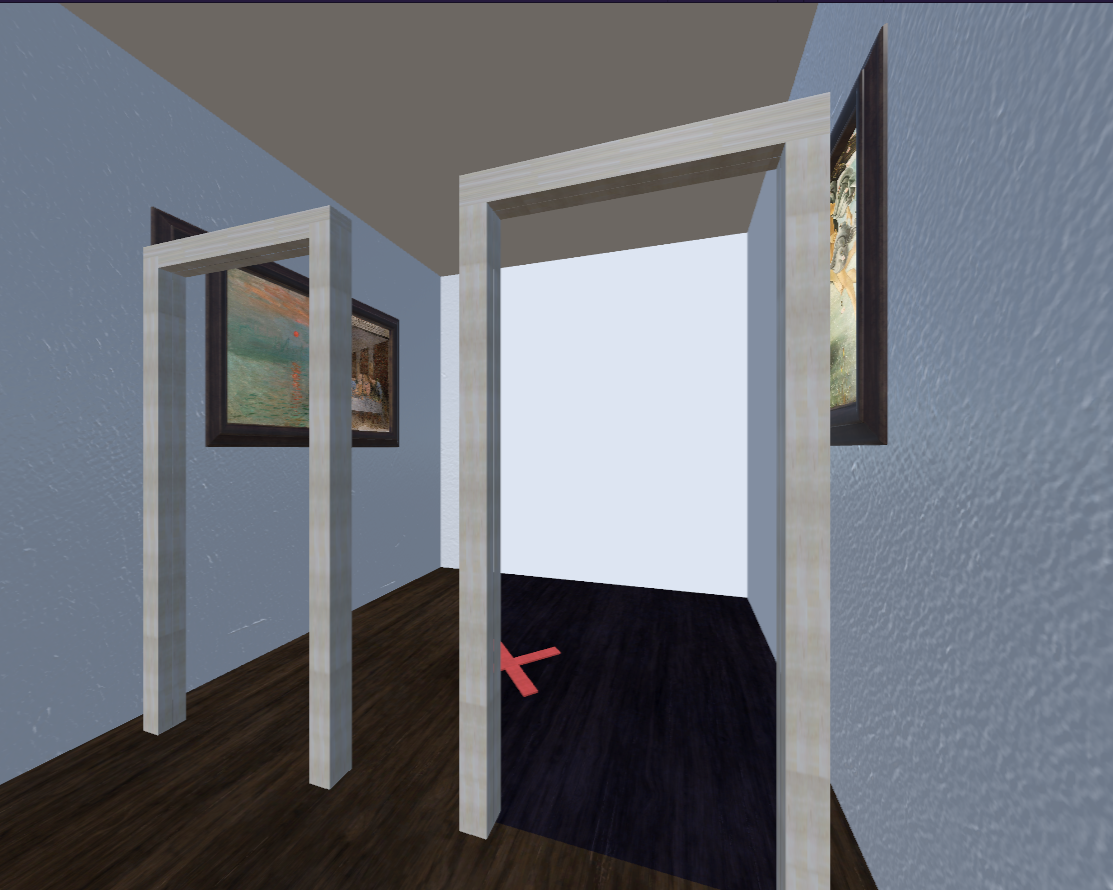
\includegraphics[width=0.6\textwidth]{NOVAthesisFiles/Images/screenshots/traditional-portal.PNG}
     \caption[The Traditional Portal.]
     {The Traditional Portal.}
     \label{fig:trad-portal-sc}
\end{figure}

A main \textit{Portal} script component handles the logic that controls the positioning of the cameras, as well as the detection and 
teleportation of a \textit{PortalTraveller} through the aforementioned trigger colliders, the rendering of the portal preview onto 
the screens and the linking between portals. The script provides a manual input of the portal that is to be linked with the portal that 
holds the script. 
With the portals linked, it is possible to calculate the positioning of the cameras using transform matrices. 
The equation for the positioning of each of the two portal cameras is:

\[
\mathbf{T}_{\text{portalCamera}} =
\mathbf{M}_{\text{thisPortal}} \cdot
\mathbf{M}_{\text{linkedPortal}}^{-1} \cdot
\mathbf{T}_{\text{eyeCamera}}
\]

where: 

\begin{itemize}
    \item $\mathbf{T}_{\text{traveller}}$ = the transform in world space of the camera correspondent with the user's eye
    \item $\mathbf{M}_{\text{linkedPortal}}^{-1}$ = inverse of the linked portal's world transform
    \item $\mathbf{M}_{\text{thisPortal}}$ = current portal's world transform
    \item $\mathbf{T}_{\text{portalCamera}}$ = the transform of the camera used to render the portal view
\end{itemize}

    
Given the interaction design of this portal type, this portal does not change states at any point during the interaction, as users only 
pass through it to go to their pertained destination.
    
\begin{figure}[t]
    \centering
     
\includegraphics[width=0.75\textwidth]{NOVAthesisFiles/Images/placeholder.pdf}
     \caption[Traditional Portal components.]
     {Traditional Portal components.}
     \label{fig:trad-portal-comp}
\end{figure}
    
\subsection{Movable Portals}
\label{sec:mov-portals}

The Movable Portal extends the functionality of the Traditional Portal, with additional features that allow it to be repositioned and 
placed within the environment, as described in Section~\ref{sec:mov-portal-design}. Figure~\ref{fig:mov-portal-sc} demonstrates the implemented interaction of the 
technique and the component structure of this portal technique is shown in Figure~\ref{fig:mov-portal-comp}.

The elements of the Traditional Portal are fully maintained: the frame, the two screens, the two cameras, and the core portal script 
on the parent object. This variant differs by introducing two handles on the portal's frame, which include colliders to enable interaction.
It also defines a valid area where the portal can be placed when grabbed. In addition to the base functionality, a dedicated
\textit{MovablePortal} script manages all behaviors related to the interaction with this portal, ensuring that its movement and placement 
follow the defined constraints.

The \textit{MovablePortal} script component defines three distinct states for this portal: \textbf{1.~Start} - when the portal is 
against the wall before being interacted - \textbf{2.~Held} - when it is being held by the user - and \textbf{3.~Placed} - when it has been 
placed in the valid area.
\begin{figure}[t]
    \centering
    \mbox{} \hfill
    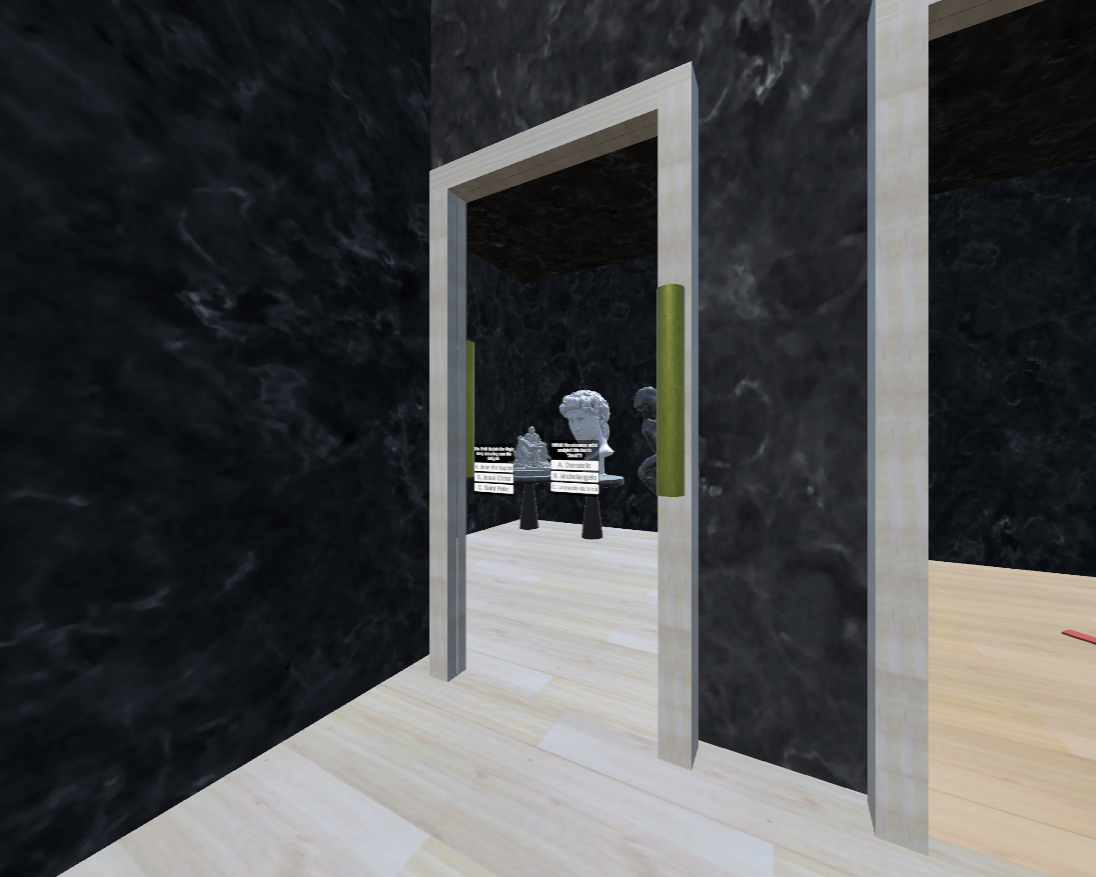
\includegraphics[width=.45\linewidth]{NOVAthesisFiles/Images/screenshots/mov-portal-a.png}
    \hfill
    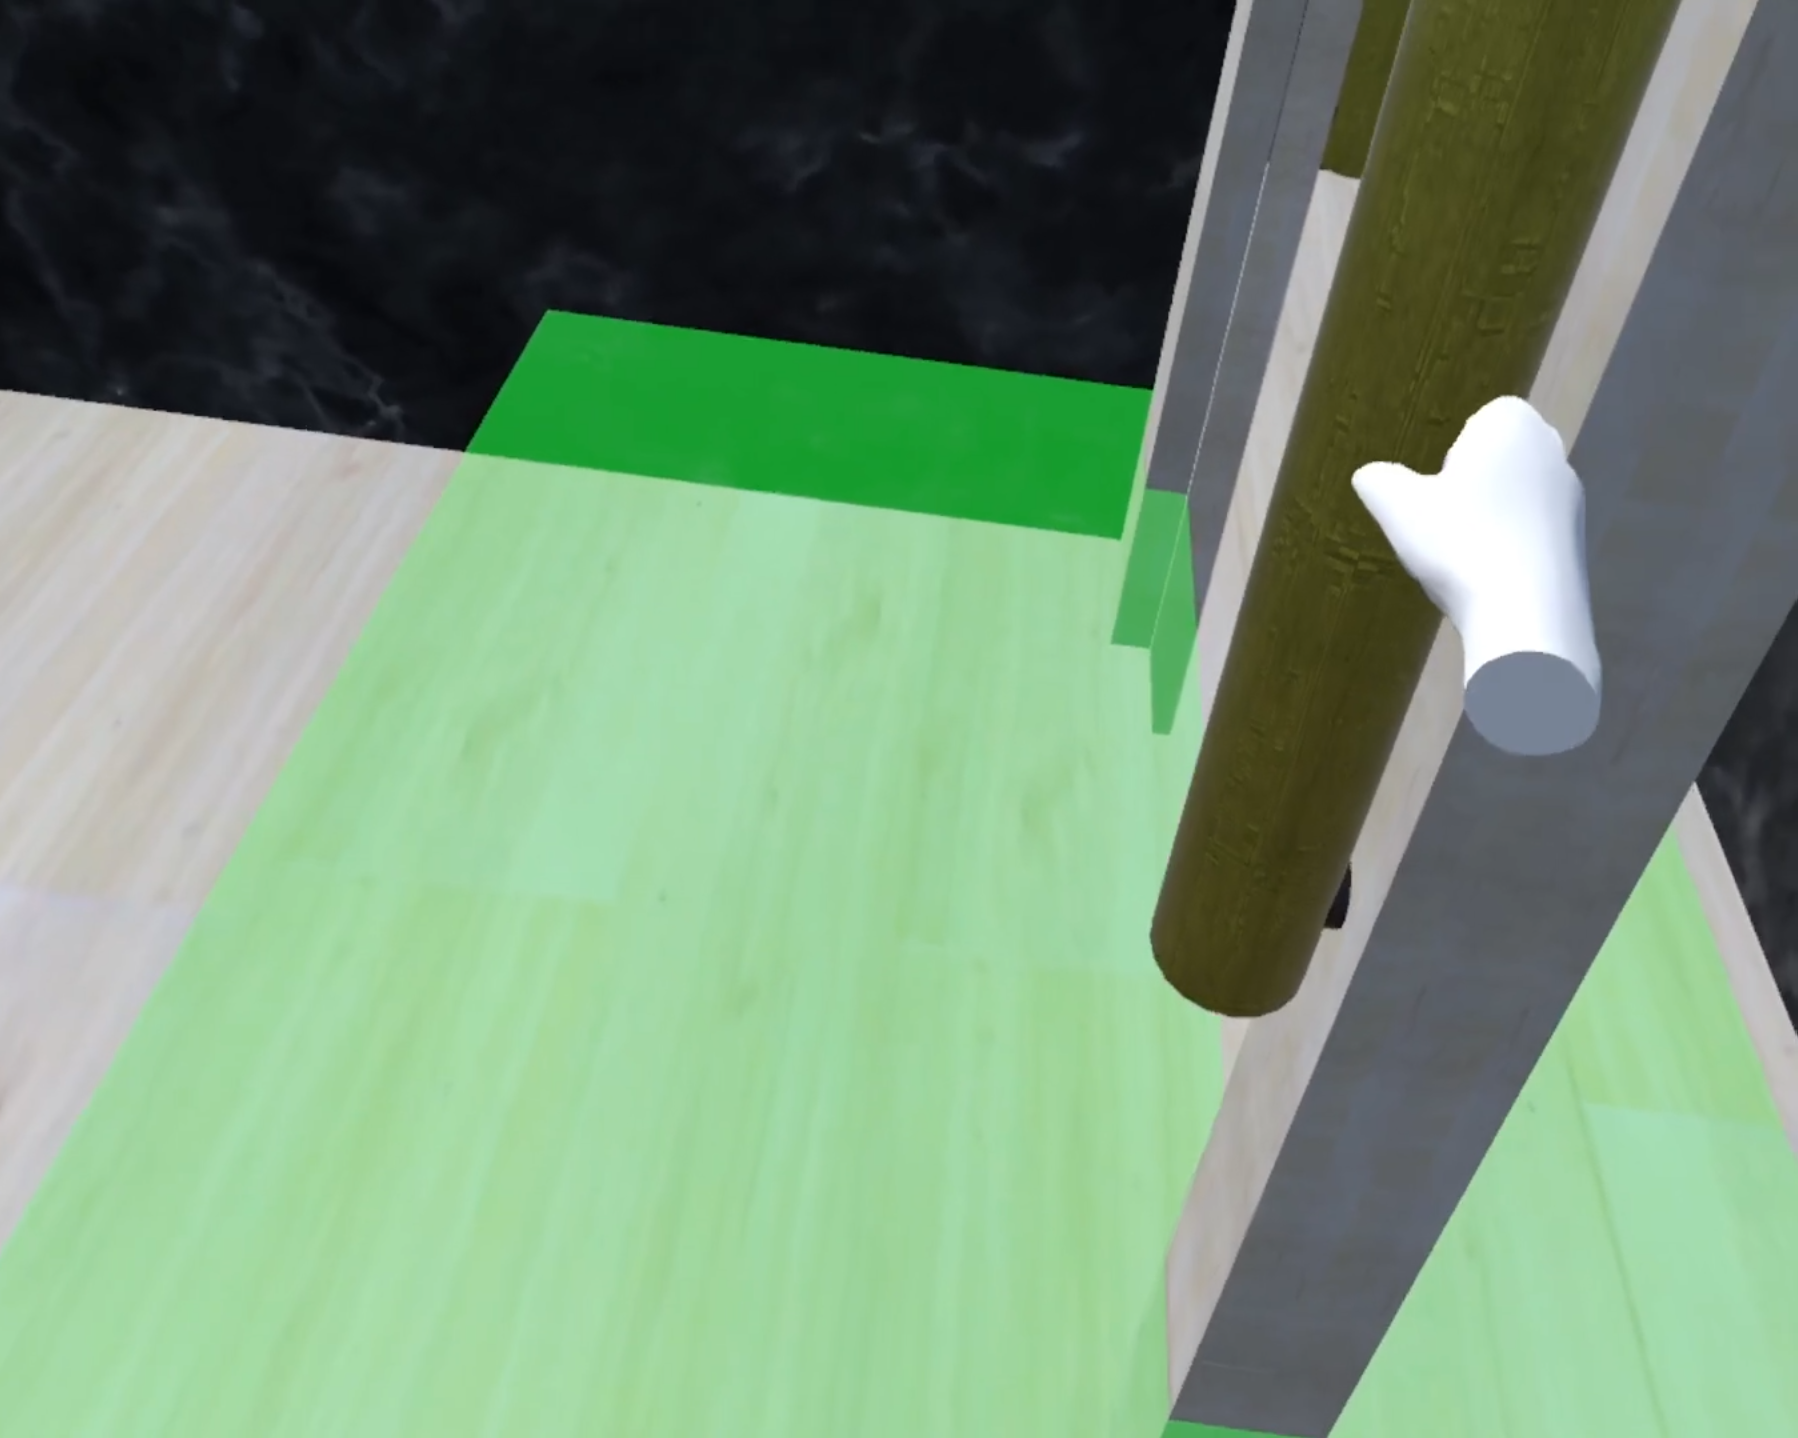
\includegraphics[width=.45\linewidth]{NOVAthesisFiles/Images/screenshots/mov-portal-b.png}
    \hfill \mbox{}
    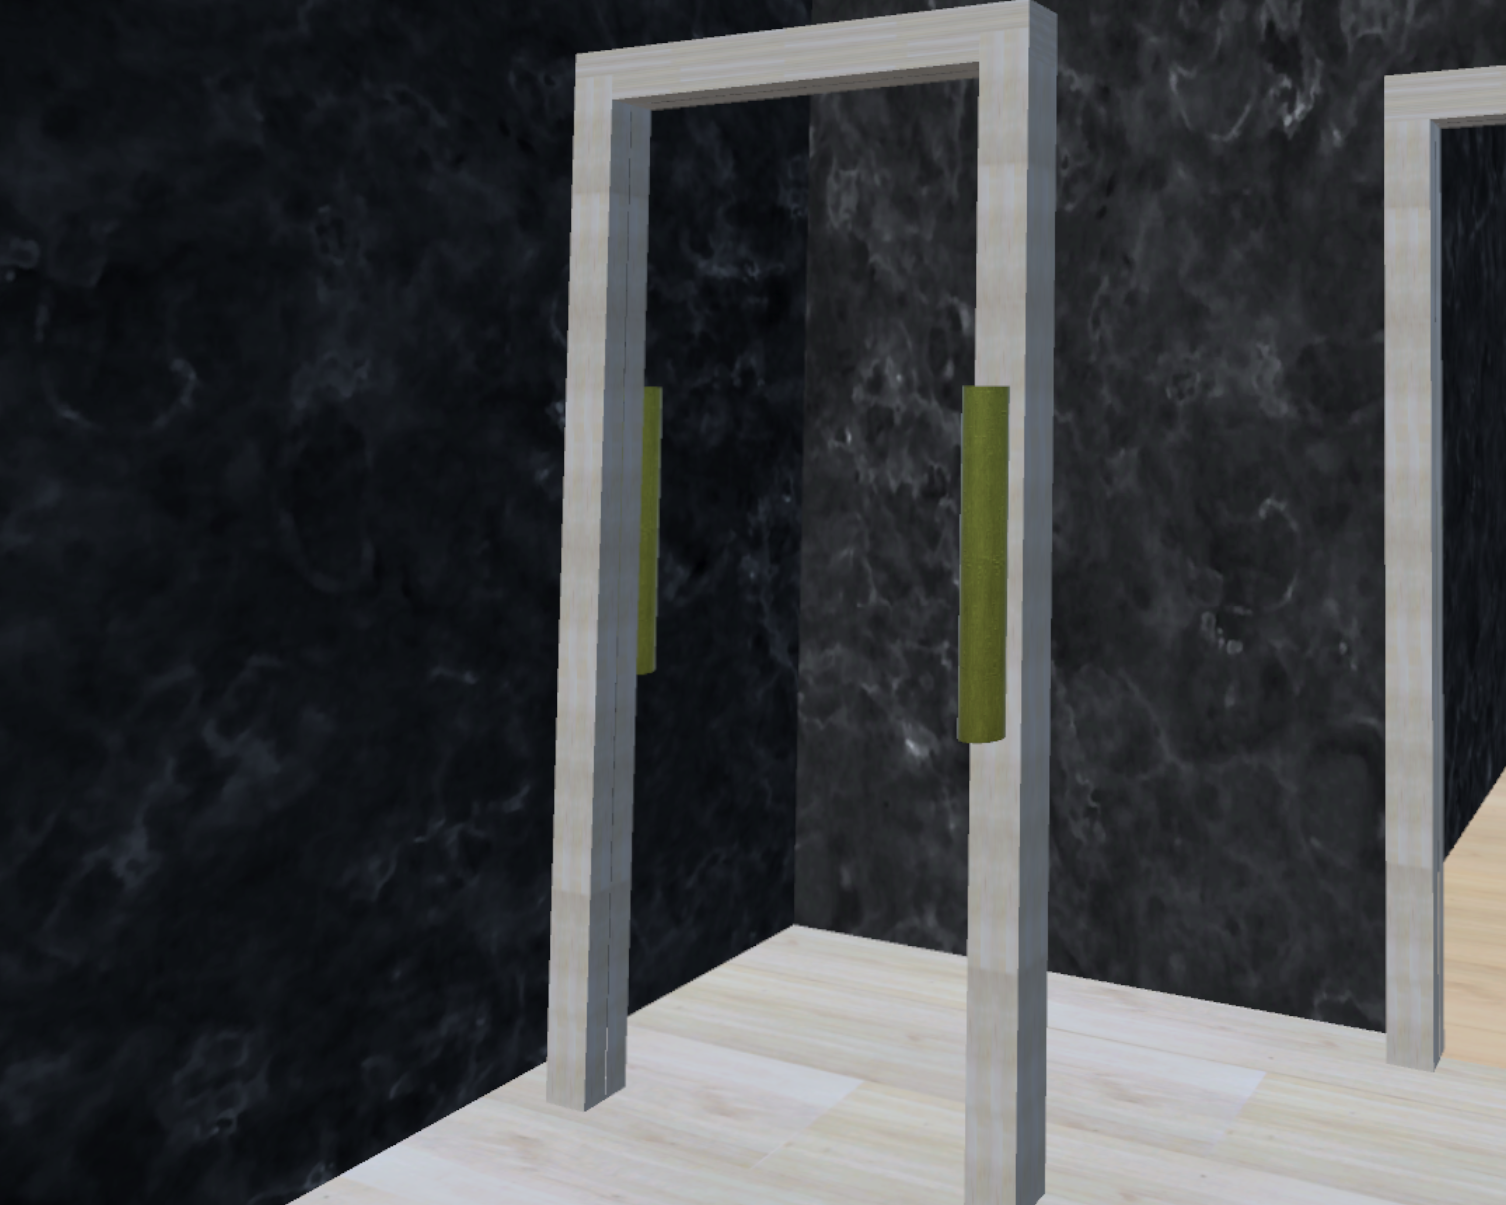
\includegraphics[width=.45\linewidth]{NOVAthesisFiles/Images/screenshots/mov-portal-c.png}
    \caption{The interaction sequence for the Movable Portal: (a) Initially, the portal is placed against the wall with a rotated continuous preview. (b) The user grabs the portal with their virtual hand through the golden-handle. A green valid area is displayed to show the user where they may place the portal. (c) The user places the portal by letting go of the golden-handle. The preview rotates to match the position of the user.}
  \label{fig:mov-portal-sc}
\end{figure}

\begin{figure}[t]
    \centering
     
\includegraphics[width=0.75\textwidth]{NOVAthesisFiles/Images/placeholder.pdf}
     \caption[Movable Portal components.]
     {Movable Portal components.}
     \label{fig:mov-portal-comp}
\end{figure}

When the portal is placed against a wall in the Start state, it renders a preview of the connected space, similar to Traditional Portals. 
However, to create the illusion of a continuous space, the preview is mirrored along the y-axis. This is effectively done by 
spinning the portal 180 degrees on the y-axis, changing the $M_{\text{thisPortal}}$ matrix from the aforementioned equation and, 
by consequence, inverting the positioning of the cameras of the linked portal. The teleport functionalities of the \textit{Portal} script 
are interrupted, preventing users from reaching the edge of their physical tracking space.

The transition to the 'Held' state happens when the user grabs the handle of the Movable Portal. Whenever a user does a grab/pinch gesture 
with their virtual hand while it is positioned within the collider of the handle, an Event is triggered, which in
turn triggers the portal's transition to the 'Held' state. 

In the 'Held' state, the position of the portal tracks the user's movement for as long as the grab gesture is maintained. 
Additionally, the valid area where the portal may be placed is also rendered and stays so for the duration of this state.
To avoid accidental teleportations, the teleport functionalities of the \textit{Portal} script remain paused, 
certifying users don't accidentally clip into the portal while holding it.

To place the portal and transition it to the 'Placed' state, the user must release it within the bounds of the valid area by ending the 
grabbing gesture. To verify if the position of the portal is valid, the following inequalities are used:
\[
P \in \text{zone} \iff 
\begin{cases} 
|\,x_p - c_x\,| \le \frac{w}{2} \\[2mm]
|\,z_p - c_z\,| \le \frac{d}{2}
\end{cases}
\]

where:
\begin{itemize}
    \item $P = (x_p, y_p, z_p)$ is the point transformed into the local space of the zone: $P' = T^{-1} P$.
    \item $C = (c_x, c_y, c_z)$ is the center of the valid zone in local coordinates.
    \item $w, d$ are the width (X-axis) and depth (Z-axis) of the box.
\end{itemize}

If let go in an invalid position, the portal returns to the 'Start' state, returning to its starting position. Otherwise, if let go in a valid 
position, the portal transitions to the 'Placed' state. When 'Placed' the linked portal matches the position of the now placed portal in the $x$ and 
$z$ axis, so that they become overlapped. The rotation of both portals are matched as well, so that the preview reverts to the way it is calculated on Traditional 
Portals, in order to achieve a seamless transition. Once this alignment is complete, the teleport functionality of the \textit{Portal} script resumes.

\subsection{Interactive Door}
\label{sec:interactive-door}

The design of the Interactive Door prioritizes naturalism, being modelled after a familiar real-world object: a door.
Its functionality extends the concept of a standard doorway by enabling dynamic interaction within the environment, 
allowing users to open and close the door at their will, manipulating the space it occupies in the environment 
in an intuitive manner. Figure~\ref{fig:int-door-sc} 
illustrates an example of the implemented interaction, while the component structure supporting this interaction is depicted 
in Figure~\ref{fig:int-door-comp}.

Designed after real-world doors, the Interactive Door is composed of a doorway completed with a panel door featuring a golden handle. 
The two screens on which the preview is rendered are behind the door, nested in the hierarchy of the door object, so that the screens position follow 
the motion the door does when opening or closing. The portal additionally includes the two cameras necessary to render the preview of the linked portal.
To manage the behavior of this portal variant, an \textit{InteractiveDoor} script was added to its parent object.

\begin{figure}[t]
  \centering
  \mbox{} \hfill
  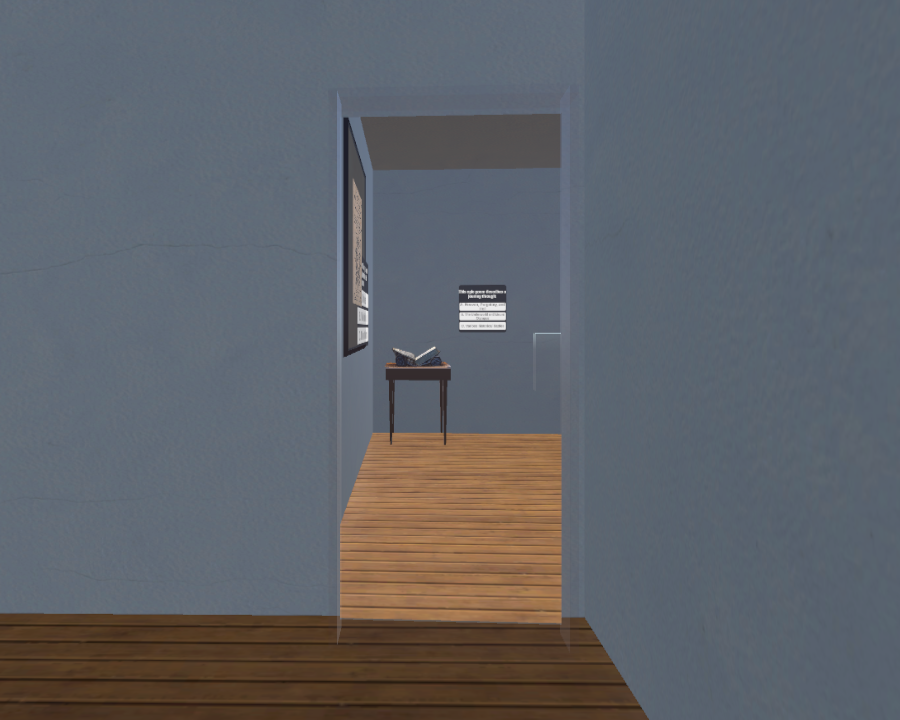
\includegraphics[width=.45\linewidth]{NOVAthesisFiles/Images/screenshots/CaptureDoorA.PNG}
  \hfill
  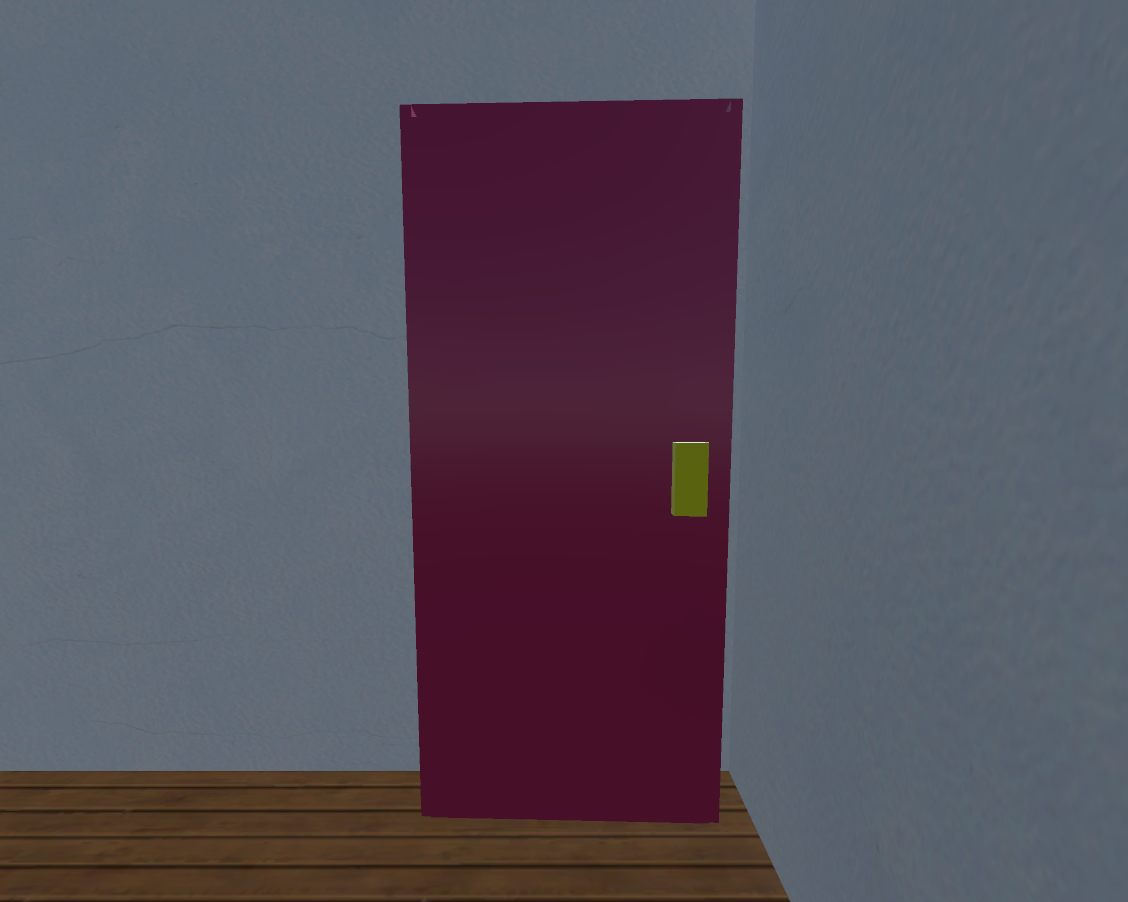
\includegraphics[width=.45\linewidth]{NOVAthesisFiles/Images/screenshots/CaptureDoorClosed.PNG}
  \hfill \mbox{}
  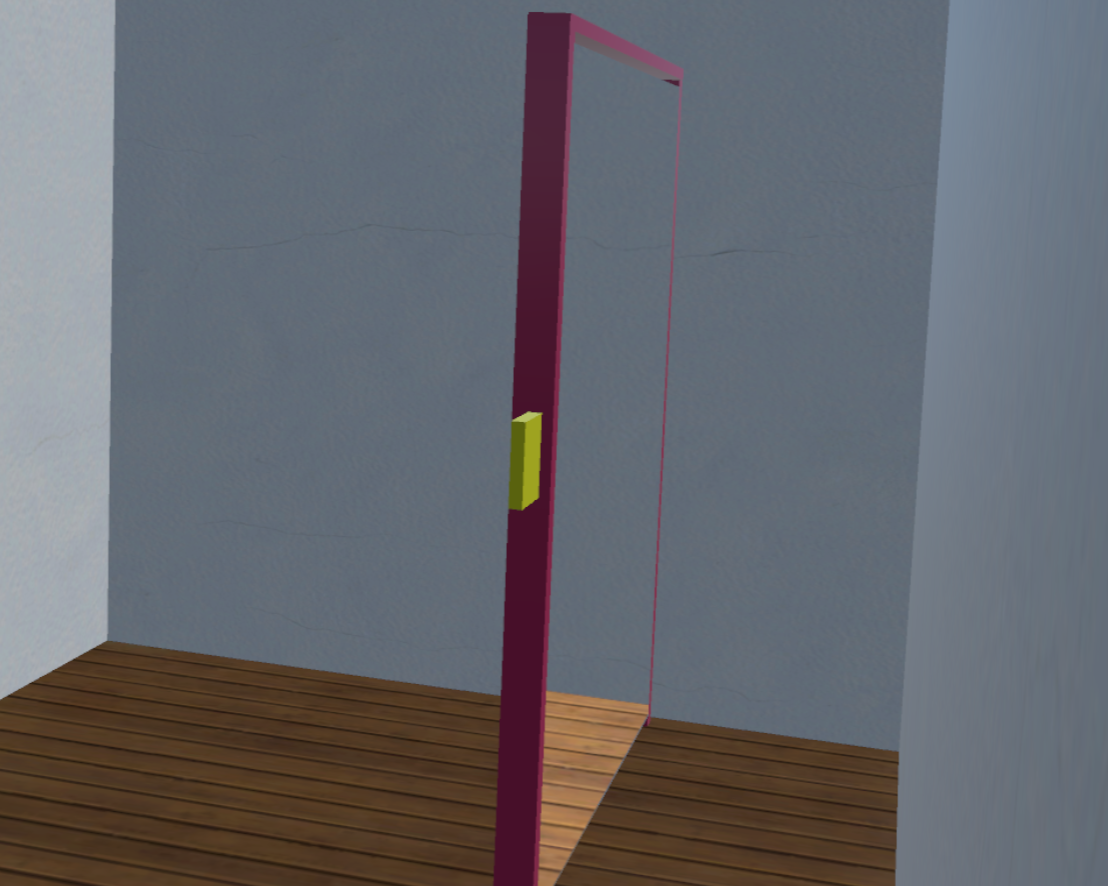
\includegraphics[width=.45\linewidth]{NOVAthesisFiles/Images/screenshots/CaptureDoorC.PNG}
  \caption{The interaction sequence for the Interactive Door: (a) From a distance, the door is transparent, providing a clear preview to aid spatial awareness. (b) As the user approaches, it becomes opaque, suggesting the need for direct interaction. (c) The user opens the door by grabbing the handle and swinging it while the portal accompanies it, creating the necessary clearance for the user to move safely into the next space.}
  \label{fig:int-door-sc}
\end{figure}

The Interactive Door may be in one of three states: \textbf{1. Closed} - the state before interaction begins, in which the door's transparency 
is dynamic - \textbf{2. Open} - the state after the user initiates the transition by opening the door - and \textbf{3. Following} - the state in 
which the portal is when the door of its linked portal is opened.

As described in Section~\ref{sec:int-door-design}, the Interactive Door is designed to allow users to perceive the connected room through 
a continuous preview of the portal behind door, with the door's transparency dynamically changing based on the proximity of the user.
Hence, when 'Closed', the portal on the Interactive Door has a reversed preview and the transparency of the door changes dynamically according 
the position of the Head of the user.
The \textit{InteractiveDoor} script receives a minimum distance, $d_{\min}$, and a maximum distance, $d_{\max}$, to calculate the $\alpha$ value 
of the transparency of the door's material using the following function:

\[
\alpha(d) =
\begin{cases}
1 & d \le d_{\min} \\[6pt]
\dfrac{d - d_{\min}}{d_{\max} - d_{\min}} & d_{\min} < d < d_{\max} \\[10pt]
0 & d \ge d_{\max}
\end{cases}
\]

where:
\begin{itemize}
  \item $\alpha(d)$ is the transparency (alpha value, ranging from $0$ to $1$),
  \item $d$ is the distance between the user's head and the door,
  \item $d_{\min}$ is the minimum distance (fully opaque for $d \le d_{\min}$),
  \item $d_{\max}$ is the maximum distance (fully transparent for $d \ge d_{\max}$).
\end{itemize}

\begin{figure}[t]
    \centering
     
\includegraphics[width=0.75\textwidth]{NOVAthesisFiles/Images/placeholder.pdf}
     \caption[Interactive Door components.]
     {Interactive Door components.}
     \label{fig:int-door-comp}
\end{figure}


When a user uses their virtual hands to grab the handle, the interacted door transitions to the 'Open' state. In the 'Open' state the door that has 
been opened by the user moves according to the pulling force the user does while still doing the grab/pinch gesture with the virtual hand. With  
a complementary hinge joint component within the hierarchy of the Interactive Door, the movement of the door can be calculated using the physics 
engine. The torque, $\tau$, which measures how strongly a force tends to make an object rotate around a pivot, is calculated by the physics engine 
through the following equation:

\[
\tau = F \cdot r \cdot \sin(\theta),
\]

where:
\begin{itemize}
  \item \(F\) is a force applied at the handle,
  \item \(r\) distance from the hinge to where the force is applied,
  \item $\theta$ angle between \(F\) and \(r\).
\end{itemize}

As the door approaches the maximum angle of $90^\circ$, the physics engine applies a constraint torque to prevent further rotation, keeping the 
door in place if more force is applied. With the Interactive Door in an 'Open' state, the \textit{Portal} script allows the teleportation of 
objects containing the \textit{PortalTraveller} script. To return the door to the 'Closed' state, the user must 
move away beyond the distance $d_{\max}$. At this point, the door plays a closing animation until fully shut, after which the dynamic transparency 
logic resumes.

As described above, when an Interactive Door transitions to the 'Open' state, its linked door automatically enters the 'Following' state. 
In this state, the linked door synchronizes its rotation with the 'Open' door, matching its angle throughout the opening motion. 
This ensures that the portals remain perfectly aligned and overlapped while the door is being opened. When the user passes through the portal, 
the doors exchange states.

\subsection{Revolving Door}
\label{sec:rev-door}

The Revolving Door portal variant explores a more continuous and guided transition, using the metaphor of a revolving door to manage both the physical and 
virtual reorientation of users. Some of the functionalities of this portal variant are shared with the Interactive Door, but it distinguishes itself 
in the designed interaction sequence. Illustrations of this interaction are present in Figure~\ref{fig:rv-door-sc} and the composition of the entity 
that makes this portal is presented in Figure~\ref{fig:rv-door-comp}.

The hierarchy of this portal variant reflects its design inspiration from revolving doors. 
The door itself is implemented as a simple 3D object with physical properties that allow it to be pushed, and a hinge joint constrains its rotation around a fixed axis. 
This door is placed within a frame composed of basic 3D objects, forming a container where the transition occurs. 
Inside this container, behind the door, lies the portal, which consists of the two screens that render the stereoscopic preview 
and the two cameras that capture the view from the linked portal.

A \textit{RevolvingDoor} script handles the logic of each of the Revolving Door's states: 
\textbf{1.~Closed} - the state before interaction begins, in which the door is still, and its transparency is dynamic - 
\textbf{2.~Open} - the state after the user initiates the transition by pushing the door - 
\textbf{3.~Following} - the state in which a portal is when the door of its linked portal is pushed.

Similarly to the Interactive Door, while in the 'Closed' state, the Revolving Door is static and has dynamic transparency according to the position 
of the user's head. The portal behind the door is then visible at a distance, displaying a rotated continuous preview of the connected room.
The dynamic transparency of the door is achieved by altering the $\alpha$ value on the color of the material of the door. The \textit{RevolvingDoor}
script takes a minimum distance where the door is fully opaque, $d_{\min}$, and a maximum distance where the door is fully transparent, $d_{\max}$,
using these values to calculate the transparency through the same formula as the Interactive Doors:

\[
\alpha(d) =
\begin{cases}
1 & d \le d_{\min} \\[6pt]
\dfrac{d - d_{\min}}{d_{\max} - d_{\min}} & d_{\min} < d < d_{\max} \\[10pt]
0 & d \ge d_{\max}
\end{cases}
\]

where:
\begin{itemize}
  \item $\alpha(d)$ is the transparency (alpha value, ranging from $0$ to $1$),
  \item $d$ is the distance between the user's head and the door,
  \item $d_{\min}$ is the minimum distance (fully opaque for $d \le d_{\min}$),
  \item $d_{\max}$ is the maximum distance (fully transparent for $d \ge d_{\max}$).
\end{itemize}

\begin{figure}[t]
  \centering
  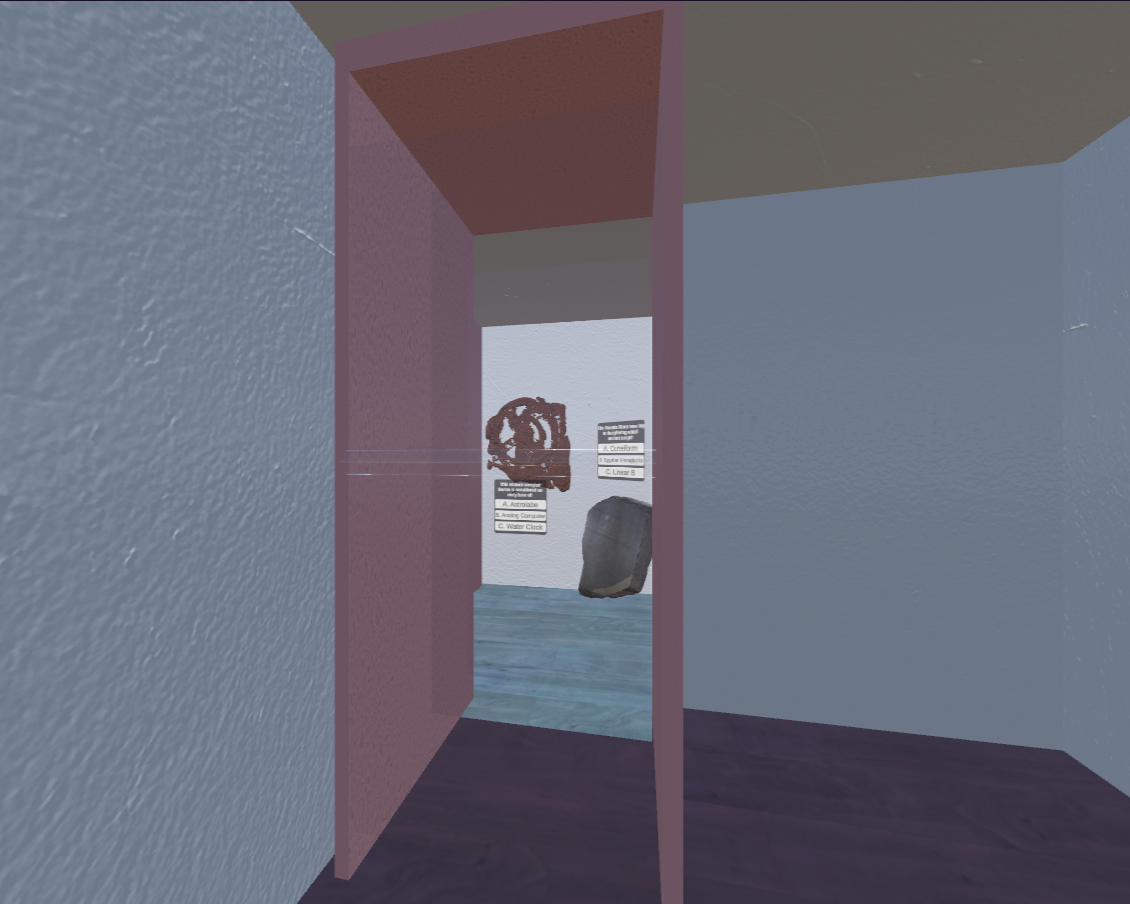
\includegraphics[width=.45\linewidth]{NOVAthesisFiles/Images/screenshots/Revolving Door Invisible.PNG}
  \hfill
  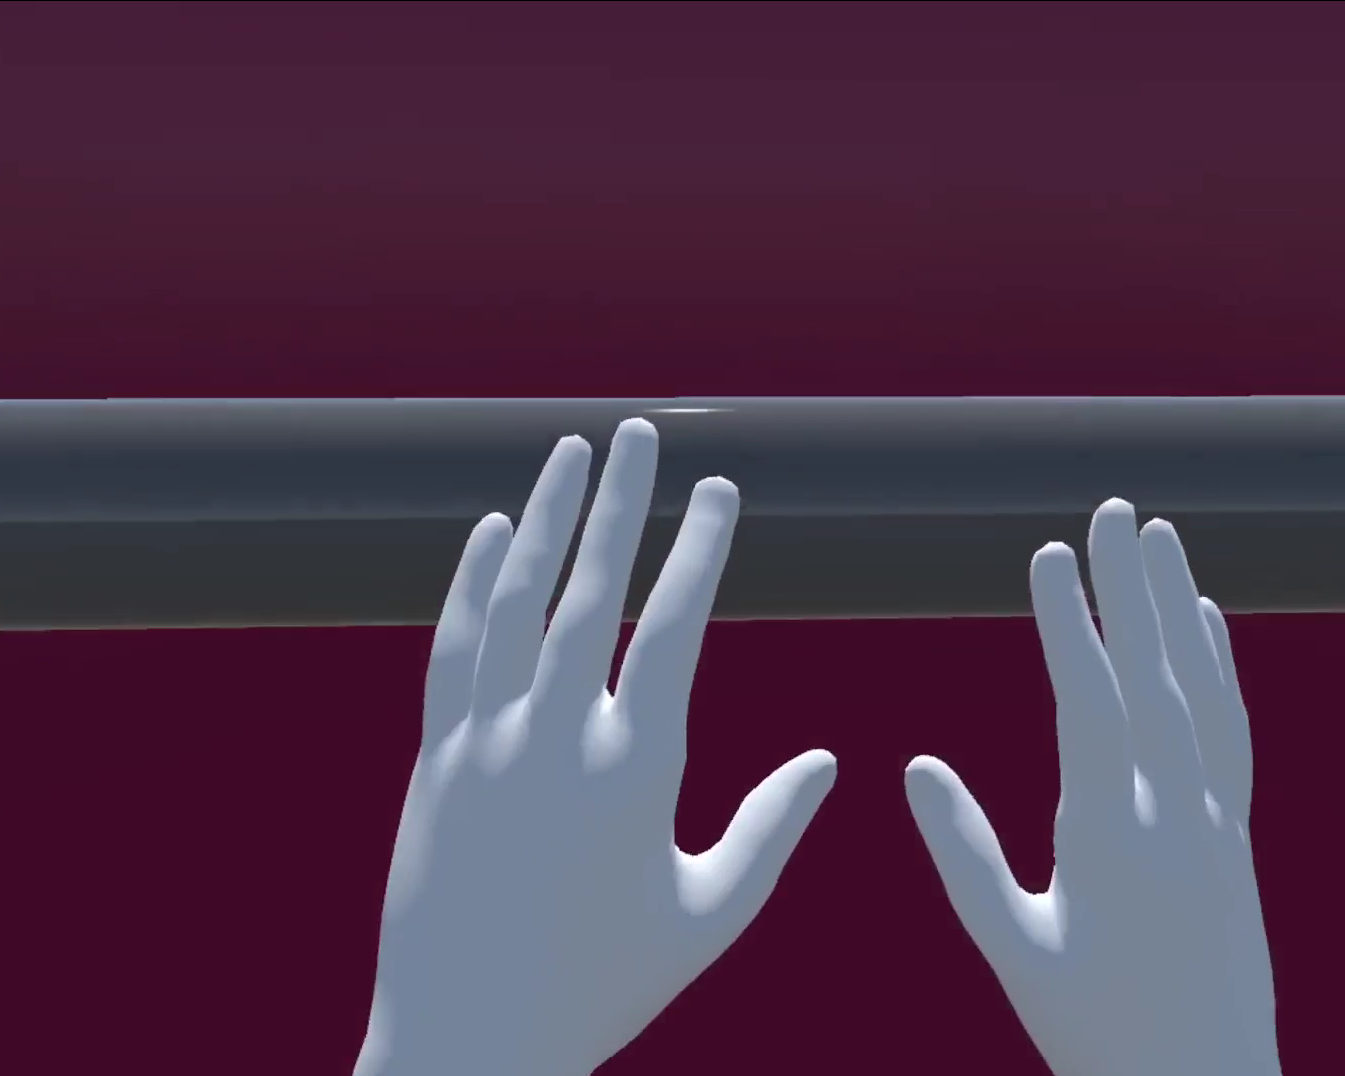
\includegraphics[width=.45\linewidth]{NOVAthesisFiles/Images/screenshots/Capture Revolving.PNG}
  \hfill
  
\includegraphics[width=.45\linewidth]{NOVAthesisFiles/Images/placeholder.pdf}
  \caption{The interaction sequence for the Revolving Door: (a) From a distance, the transparent panels provide a preview of the next room. 
  (b) The user initiates the transition by walking into a compartment, pushing the door.
  (c) After pushing the door and completing a 180-degree turn, the user comes out on the other side. 
  }
  \label{fig:rv-door-sc}
\end{figure}

For this portal the transition to the 'Open' state occurs when the door becomes fully opaque, when the user reaches the minimum distance, $d_{\min}$.
In this state the portal reverses the preview back and rotates to a perpendicular position, so the user transitions to the next room mid-push.
Although the force applied to the door is different, since the user pushes the door instead of pulling it, the formula to calculate the 
torque applied to the door is the same as the Interactive Door:

\[
\tau = F \cdot r \cdot \sin(\theta),
\]

where:
\begin{itemize}
  \item \(F\) is a force applied at the handle,
  \item \(r\) distance from the hinge to where the force is applied,
  \item $\theta$ angle between \(F\) and \(r\).
\end{itemize}

The Revolving Door's return to the 'Closed' state is gradual. As soon as the user distances itself from the door at the minimum distance, $d_{\min}$,
the portal returns to the parallel position, with a continuous preview. The full 'Closed' state is only reached when the user distances themselves 
at the maximum distance, $d_{\max}$, where the door becomes fully transparent. When the door becomes invisible its angular speed, $\omega$,
is set to 0, guaranteeing that the rotation of the door is stopped, and it's position and rotation are set back as default. At this point the door 
becomes fully 'Closed'.

As mentioned, the Revolving Door enters the 'Following' state when the linked door is 'Open'. In this state the rotation of the door is synchronized
with the rotation of the linked door. When the user passes through the portal, the doors exchange states.

\begin{figure}[t]
    \centering
     
\includegraphics[width=0.75\textwidth]{NOVAthesisFiles/Images/placeholder.pdf}
     \caption[Revolving Door components.]
     {Revolving Door components.}
     \label{fig:rev-door-comp}
\end{figure}

\section{UI}
\label{sec:ui}

A \glsfirst{UI} was implemented to support both participants and experimenters throughout the case study. 
Participant tasks relied on in-world \gls{UI} elements, which encouraged exploration of the \gls{VE} and enabled 
the evaluation of the locomotion techniques. A separate researcher interface, shown only on the desktop monitor, 
provided controls to manage the study's flow and record participant input.


\subsection{Panels}
\label{sec:panels}

As described in Section~\ref{sec:case-study}, the case study relies on exploratory tasks associated 
with the artworks exhibited in the virtual museum, as well as evaluation tasks that should occur within the \gls{VE}. 
To present these tasks to the users and collect their responses, interactive \gls{UI} Panels were implemented within the environment.
All \gls{UI} Panels have a dark base panel where text is displayed. Panels with interactive functionality integrate the use of buttons that 
are selectable using the virtual hands of the player.

The most common example of interactable \gls{UI} throughout the \gls{VE} are the quizes associated with each exposition item of the museum \gls{VE}. 
These panels display the question as text with three selectable buttons for the multiple possible answers, A, B and C~(Figure~\ref{fig:quiz-panel}).
Once one of the options is selected, the option becomes either green or red, if it is a correct or incorrect option, respectively. After selecting 
an option, a second curious fact panel is instantiated with only text describing the curious fact.

\begin{figure}[t]
    \centering
     
\includegraphics[width=0.75\textwidth]{NOVAthesisFiles/Images/placeholder.pdf}
     \caption[Quiz UI panels used for the museum exposition items.]
     {Quiz UI panels used for the museum exposition items.}
     \label{fig:quiz-panel}
\end{figure}

\begin{figure}[b]
    \centering
     
\includegraphics[width=0.75\textwidth]{NOVAthesisFiles/Images/placeholder.pdf}
     \caption[UI panels used for in-world Likert scale evaluations.]
     {UI panels used for in-world Likert scale evaluations.}
     \label{fig:likert-scale-ui}
\end{figure}
At the end of each section of the study, users are tasked to evaluate the portal variant they used. For this, more interactable \gls{UI} panels 
were developed, allowing users to perform this task immediately after experiencing the portal technique, without leaving the \gls{VE} (Figure~\ref{fig:likert-scale-ui}).
This \gls{UI} panel displays an affirmation in text and bellow buttons from the number 1 to 7 fill the panel horizontally, so users may rate 
how much they agree with the statement according to a 7-point Likert scale (1=strongly disagree and 7=strongly agree). A 'Next' button permits 
users to go to the next affirmation, and a submit button saves the answers provided by users to a file.

Before these panels, for the pointing task, a \gls{UI} panel displaying text and an image was also developed. The text describes the requirements 
of the pointing task, with the image exemplifying the object to be pointed towards~(Figure~\ref{fig:pointing-task-ui}).


\begin{figure}[t]
    \centering
     
\includegraphics[width=0.75\textwidth]{NOVAthesisFiles/Images/placeholder.pdf}
     \caption[UI panels used for in-world Likert scale evaluations.]
     {UI panels used for in-world Likert scale evaluations.}
     \label{fig:pointing-task-ui}
\end{figure}

\subsection{Researcher UI}
\label{sec:gui}

To give experimenters control over the course of the study, a researcher \gls{UI} was developed. 
It consists on two buttons and a status text display that are displayed in the top left corner of the screen (Figure~\ref{fig:researcher-ui}).
This \gls{UI} is only displayed on the monitor of the \gls{PC} it is being run on, not being visible for the \gls{VR} user wearing the \gls{HMD}.

\begin{figure}[b]
    \centering
     
\includegraphics[width=0.75\textwidth]{NOVAthesisFiles/Images/placeholder.pdf}
     \caption[UI used by researchers during the experience.]
     {UI used by researchers during the experience.}
     \label{fig:likert-scale-ui}
\end{figure}

The \textit{End Section} button is used to end the section the user is in to proceed to the next section. Logic wise, when this button is pressed 
it instantiates the previously mentioned panels at the starting room of the current section. 

The \textit{Toggle Pointing Ray} button is used for the pointing task, as it instantiates a pointing ray in the user's right virtual 
hand~(Figure~\ref{fig:pointing-ray}). Upon selection, the \textit{Status} feedbacks this change by displaying 'ON', and the \textit{Toggle Pointing 
Ray} button is replaced with a \textit{Disable Pointing Ray} button. The logic of the button is changed, 
as when it is pressed the system stores the position and direction of the toggled pointing ray in a file, before the ray is deleted.

\begin{figure}[t]
    \centering
     
\includegraphics[width=0.75\textwidth]{NOVAthesisFiles/Images/placeholder.pdf}
     \caption[The Pointing Ray used for the pointing task.]
     {The Pointing Ray used for the pointing task.}
     \label{fig:likert-scale-ui}
\end{figure}


\section{Summary}
\label{sec:summary}
\todo{Completar de acordo como ficar no final}
 


